\chapter{Implementaci\'on}\label{chapter:code}

En este capítulo se discutirá acerca de la implementación del algoritmo \ref{al:PRA} presentado en el capítulo \ref{chapter:scheme} y del esquema final de la restauraci\'on presentado en el epígrafe \ref{sec:final_scheme}. El c\'odigo fuente de la implementaci\'on puede consultarse en el siguiente repositorio: \url{https://github.com/danielgpz/image-inpainting-sop.git}.

\section{Tecnolog\'ias utilizadas}
Todos los algoritmos y el c\'odigo fuente en general ha sido implementado en el lenguaje de programaci\'on \texttt{Python3}, específicamente en su versi\'on \texttt{python 3.7.3}. Para el trabajo con los archivos de im\'agenes digitales, como son las operaciones de \textit{lectura}\footnote{Operaci\'on de cargar determinados datos en un disco duro o dispositivo de almacenamiento hacia la memoria \textbf{RAM}} y \textit{escritura}\footnote{Operaci\'on inversa de la lectura, copiar determinados datos de la memoria hacia el dispositivo de almacenamiento} se us\'o la librer\'ia \texttt{OpenCV}\footnote{Por sus siglas en ingles \textit{Open Source Computer Vision Library}: librer\'ia para visi\'on por computadoras de c\'odigo abierto} en su versi\'on \texttt{cv2 4.2.0}. \texttt{OpenCV} es un \textit{software} librer\'ia de c\'odigo abierto\footnote{D\'igase de aquellos programas cuyo c\'odigo fuente no est\'a oculto o encriptado. Cualquier usuario es libre de verificarlo y contribuir al mismo} que se utiliza para visi\'on por computadoras e Inteligencia Artificial. La misma contiene m\'as de $2500$ algoritmos optimizados que comprenden tanto los cl\'asicos como los del estado del arte en los dos campos anteriormente mencionados. Utilizando los m\'etodos \fbox{\texttt{cv2.imread}} y \fbox{\texttt{cv2.imwrite}} de esta librer\'ia se logra la lectura y la escritura respectivamente de las im\'agenes digitales, y permiten adem\'as obtener la representaci\'on matricial asociada. Ambas funciones soportan el uso de la mayor\'ia de los formatos para imágenes de mapa de bits como son \texttt{.jpg}, \texttt{.jpeg}, \texttt{.png}, \texttt{.tif}, \textit{etc}. Tambi\'en cuenta con la opción de interpretar una imagen ya sea en \RGB o en escala de grises.

Para el trabajo con matrices, vectores y otros elementos y operaciones matem\'aticas se hizo uso de librer\'ia \texttt{NumPy} en su versi\'on \texttt{numpy 1.17.4}. Quizás es considerada la librer\'ia m\'as ampliamente usada del paquete científico de \texttt{Python}. La misma provee las herramientas para tratar con las matrices obtenidas mediante \texttt{OpenCV} y adem\'as facilita realizar transformaciones y operaciones tanto elementales como avanzadas. Adem\'as de las matrices, se usa tambi\'en el m\'odulo \fbox{\texttt{numpy.random}} \'util para el trabajo con variables aleatorias. \texttt{NumPy} es r\'apida y eficiente, conocida por estar mayormente implementada en el lenguaje \texttt{C} lo que ayuda a evitar los procesos lentos y cargados en memoria t\'ipicos de \texttt{Python}.

Se hace uso tambi\'en de otra de las librer\'ias m\'as famosas del paquete científico, es el caso de \texttt{SciPy}. La versión usada es \texttt{scipy 1.3.2}. De esta se toma el m\'odulo \fbox{\texttt{scipy.interpolate}} el cual contiene, entre otras, una funci\'on para realizar la interpolaci\'on por \textit{splines} c\'ubicos. Finalmente, con el objetivo de optimizar el tiempo de ejecuci\'on de los esquemas y algoritmos presentados en el Cap\'itulo \ref{chapter:scheme} se utiliza el m\'odulo \texttt{multiprocessing}. Este paquete soporta la ejecuci\'on de procesos concurrentes, de una forma similar al m\'odulo \texttt{threading}, con la gran diferencia de que estos procesos s\'i corren en diferentes n\'ucleos de la \textbf{CPU}\footnote{Por sus siglas en ingl\'es \textit{Central Processing Unit}: unidad central de procesamiento} \cite{enwiki:cpu}. Resulta de utilidad este m\'odulo para lograr la paralelizaci\'on de los esquemas de restauraci\'on presentados, que tal como sus gr\'aficos muestran (figuras \ref{fig:subimage_scheme} y \ref{fig:final_scheme}), sus partes pueden ser realizadas de forma independiente.

\section{El m\'odulo \texttt{ImageInpainting}}

Para lograr una mejor organizaci\'on y diseño de la implementaci\'on del esquema de restauraci\'on, la misma se creo en forma de m\'odulo local de \texttt{Python}, el cual se nombr\'o \texttt{ImageInpainting}. Cada una de sus funcionalidades fueron encapsuladas en 3 archivos distintos:
\begin{itemize}
	\item \texttt{images.py}: este archivo contiene los m\'etodos para la lectura y escritura de las im\'agenes digitales y su conversi\'on a matrices de tipo \texttt{numpy.ndarray}.
	\item \texttt{pra.py}: solo contiene un \'unico m\'etodo con la implementaci\'on del algoritmo \ref{al:PRA}.
	\item \texttt{inpainting.py}: el mismo contiene la implementaci\'on de una clase para modelar el concepto de imagen corrupta o con p\'ixeles faltantes. Adem\'as contiene las implentaciones del operador $\H$ y la funci\'on de distancia $\omega$. 
\end{itemize}

A continuaci\'on se da una explicaci\'on m\'as en profundidad por cada uno de los archivos. Comenzando por \texttt{images.py}, en este se encuentran las siguientes funciones con sus respectivas características:
\begin{itemize}
	\item M\'etodo que por medio de \texttt{cv2.imread} lee la imagen digital del disco duro, y la transforma a uno o tres arreglos bidimensionales de \texttt{numpy}.
	
	\fbox{\lstinline|read_image_as_arrays(location: str, rgb=False, dtype=int)|}
	\begin{itemize}
		\item \texttt{location}: tipo \texttt{str}, direcci\'on donde se almacena la im\'agen a leer en el disco.
		\item \texttt{rgb}: tipo \texttt{bool}, indica si la imagen debe ser le\'ida como \RGB o escala de grises. En el primer caso, se generar\'an 3 arreglos uno por cada canal. En el caso de la escala de grises, un \'unico arreglo. Valor por defecto: \texttt{False}.
		\item \texttt{dtype}: tipo \texttt{type}, tipo datos con que se interpretar\'an los p\'ixeles. Usar \texttt{int} para el intervalo usual de $[0,\; 255]$. Usar \texttt{bool} para interpretar la imagen como una m\'ascara. Valor por defecto: \texttt{int}.
	\end{itemize}
	\underline{Retorna}: una tupla de arreglos, cada arreglo representando uno de los canales de la imagen, 3 para \texttt{rgb=True} y 1 para \texttt{rgb=False}.
	
	\item M\'etodo que por medio de \texttt{cv2.imread} lee la imagen digital del disco duro, y la interpreta como una m\'ascara.
	
	\fbox{\lstinline|read_image_as_mask(location, true_value=0)|}
	\begin{itemize}
		\item \texttt{location}: tipo \texttt{str}, direcci\'on donde se almacena la im\'agen m\'ascara en el disco.
		\item \texttt{true\_value}: tipo \texttt{int}, indica el valor de los p\'ixeles que se tomar\'an como \texttt{True} en la m\'ascara que se retorna. Valor por defecto \texttt{0}.
	\end{itemize}
	\underline{Retorna}: un arreglo bidimensional de booleanos, la m\'ascara leída.
	
	\item 	M\'etodo que, usando \texttt{cv2.imwrite}, almacena la imagen digital en el disco duro. Dicha imagen es la representada por el par\'ametro \texttt{arrays}.
	
	\fbox{\lstinline|save_arrays_as_image(arrays: tuple, location: str, rgb=False)|}
	\begin{itemize}
		\item \texttt{arrays}: tipo \texttt{tuple}, tupla de uno o tres arreglos bidimensionales que representan los canales de la imagen a alamacenar.
		\item \texttt{location}: tipo \texttt{str}, direcci\'on que indica donde debe ser almacenada la imagen en el disco duro.
		\item \texttt{rgb}: tipo \texttt{bool}, tipo de imagen a almacenar, en caso de \texttt{True} se usan los tres arreglos representando en ese orden cada uno de los canales \RGB. Si no, se toma solo el primero. Valor por defecto: \texttt{False}. 
	\end{itemize}
	\underline{Retorna}: \texttt{None}. No tiene valor de retorno, se considera un m\'etodo \textit{void}.
\end{itemize}

En el caso del archivo \texttt{pra.py}, como se mencion\'o, este contiene la implementaci\'on del algoritmo \ref{al:PRA}. El cual tiene la signatura siguiente:
\begin{itemize}
	\item M\'etodo implementado a partir del pseudoc\'odigo del algoritmo \ref{al:PRA}.
	
	\fbox{\lstinline|patch_reordering(shape: tuple, patches, B: int, epsilon: float, omega)|}
	\begin{itemize}
		\item \texttt{shape}: tipo \texttt{tuple}, tupla de 2 elementos que denota la dimensi\'on de cada subimagen, en otras palabras ($N_1 - \sqrt{n} + 1)$ y $(N_2 - \sqrt{n} + 1)$.
		\item \texttt{patches}: tipo \texttt{numpy.ndarray}, arreglo bidimensional que representa la matriz $X^\intercal$, cada fila es un parche vectorizado. Los parches se toman columna por columna de arriba hacia abajo.
		\item \texttt{B}: tipo \texttt{int}, entero que representa el tamaño de la vecindad a explorar en cada iteraci\'on.
		\item \texttt{epsilon}: tipo \texttt{float}, n\'umero de punto flotante que se atribuye a $\epsilon$.
		\item \texttt{omega}: tipo \texttt{function}, funci\'on que toma 2 par\'ametros de tipo \texttt{numpy.array} y retorna un \texttt{float} que es la distancia entre esos 2 arreglos que contienen los elementos de 2 parches vectorizados. Equivalente de la funci\'on $\omega$.
	\end{itemize}
	\underline{Retorna}: una tupla de 2 arreglos, el primero contiene los \'indices que definen la permutaci\'on generada y el segundo los de la permutaci\'on inversa.
\end{itemize}

Finalmente el archivo principal \texttt{inpainting.py}, el cual contiene las funcionalidades para realizar el esquema completo de la restauraci\'on, haciendo uso de los m\'etodos implementados en \texttt{images.py} y \texttt{pra.py}. En el mismo se encuentran las implementaciones para el operador $\H$ y la funci\'on de distancia entre parches $\omega$.
\begin{itemize}
	\item M\'etodo para calcular la distancia entre dos parches seg\'un (\ref{eq:omega}).
	
	\fbox{\lstinline|mean_of_squared_differences(patch1: array, patch2: array)|}
	\begin{itemize}
		\item \texttt{patch1}, \texttt{patch2}: tipo \texttt{numpy.array}, arreglos que representan un parche en forma de vector
	\end{itemize}
	\underline{Retorna}: un flotante, la distancia entre \texttt{parch1} y \texttt{patch2}, \texttt{-1} en caso de ser disjuntos en cuanto a sus p\'ixeles no faltantes.
	
	\item M\'etodo para aplicar el operador de suavidad usando un \textit{spline} c\'ubico.
	
	\fbox{\lstinline|cubic_spline(signal: array, mask: array)|}
	\begin{itemize}
		\item \texttt{signal}: tipo \texttt{numpy.array}, arreglo de elementos que representa una señal a interpolar.
		\item \texttt{mask}: tipo \texttt{numpy.array}, arreglo de elementos booleanos, de mismo tamaño que \texttt{signal} y contiene \texttt{False} en aquella posiciones donde ocurre un elemento faltante de \texttt{signal}.
	\end{itemize}
	\underline{Retorna}: un arreglo de mismo tamaño que \texttt{signal} resultado de la interpolaci\'on en cada una de las posciones del arreglo \texttt{signal}.
\end{itemize}
Para modelar el concepto de una imagen con p\'ixeles faltantes se implement\'o:
\begin{lstlisting}
class CorruptedImage:
	def __init__(self, location: str, mask=None, rgb=False, 
				corrupt_prob=4/5): ...
	
	def save(self, location: str): ...
	
	def inpainting(self, K=10, sqrt_n=16, B=9, epsilon=10**4,
				H=cubic_spline, omega=mean_of_squared_differences): ...
\end{lstlisting}
\begin{itemize}
	\item M\'etodo inicializador de una instancia de la clase \texttt{CorruptedImage}
	
	\fbox{\lstinline|__init__(self, location: str, mask=None, rgb=False, corrupt_prob=4/5)|}
	\begin{itemize}
		\item \texttt{location}: tipo \texttt{str}, direcci\'on en el disco duro de la imagen digital a recuperar. Los canales de la misma se obtienen mediante \texttt{read\_image\_as\_arrays} y se almacenan en el atributo \texttt{self.channels}.
		\item \texttt{mask}: tipo \texttt{numpy.ndarray}, arreglo booleano bidimensional de mimas dimensi\'on que la imagen cargada. M\'ascara que indica con \texttt{False} los p\'ixeles faltantes. Se almacena en el atributo \texttt{self.mask}. Valor por defecto: \texttt{None}.
		\item \texttt{rgb}: tipo \texttt{bool}, par\'ametro que indica si la imagen debe ser cargada como \RGB o escala de grises. Valor por defecto: \texttt{False}.
		\item \texttt{corrupt\_prob}: tipo \texttt{float}, valor en el intervalo $[0,\; 1]$. En caso de que \texttt{mask} sea \texttt{None}, se genera una m\'ascara de forma aleatoria asignando \texttt{False} en cada posici\'on con probabilidad de dicho valor. Valor por defecto: \texttt{4/5}. 
	\end{itemize}
	\underline{Retorna}: la instancia creada.
	
	\item M\'etodo de instancia para almacenar el estado actual de la imagen en el disco duro.
	
	\fbox{\lstinline|save(self, location: str)|}
	\begin{itemize}
		\item \texttt{location}: tipo \texttt{str}, direcci\'on en el disco duro d\'onde almacenar la imagen. 
	\end{itemize}
	\underline{Retorna}: \texttt{None}, es un m\'etodo \textit{void}.
	
	\item M\'etodo para realizar el esquema de restauraci\'on (figura \ref{fig:final_scheme}) a cada uno de los canales almacenados en el atributo de la instancia \texttt{self.channels}.
	
	\begin{lstlisting}
inpainting(self, K=10, sqrt_n=16, B=9, epsilon=10**4, H=cubic_spline,
			omega=mean_of_squared_differences)
	\end{lstlisting}
	\begin{itemize}
		\item \texttt{K}: tipo \texttt{int}, cantidad de permutaci\'ones diferentes a usar en el esquema, las cuales se obtienen usando el m\'etodo \texttt{patch\_reordering}. Valor por defecto \texttt{10}.
		\item \texttt{sqrt\_n}: tipo \texttt{int}, valor de $\sqrt{n}$ que indica que los parches tienen dimensi\'on $\sqrt{n} \times \sqrt{n}$. Valor por defecto \texttt{16}.
		\item \texttt{B}: tipo \texttt{int}, tamaño de la vecindad a usar en los llamados al m\'etodo \texttt{patch\_reordering}. Valor por defecto \texttt{9}.
		\item \texttt{epsilon}: tipo \texttt{float}, valor de $\epsilon$ a usar en los llamados al m\'etodo \\\texttt{patch\_reordering}. Valor por defecto \texttt{10000}.
		\item \texttt{H}:tipo \texttt{function}, m\'etodo que recibe dos arreglos y retorna una tercero, todos de igual tamaño. El arreglo retornado debe ser el resultado de aplicarle determinado operador de suavidad a la señal representada por el primero, usando el segundo como m\'ascara para definir los elementos corruptos. Valor por defecto, m\'etodo \texttt{cubic\_spline}.
		\item \texttt{omega}: tipo \texttt{function}, m\'etodo que representa la funci\'on $\omega$ a usar en los llamados al m\'etodo \texttt{patch\_reordering}. Valor por defecto, el m\'etodo \texttt{mean\_of\_squared\_differences}.
	\end{itemize}
	\underline{Retorna}: \texttt{None}, es un m\'etodo \textit{void}.
\end{itemize}

\textquestiondown C\'omo usar el m\'odulo \texttt{ImageInpainting}? Supongamos que contamos con la imagen \texttt{woman\_blonde.tif} y otra de igual dimensiones en forma de m\'ascara \texttt{mask.tif}. Ver figura \ref{fig:woman_blonde}.
\begin{figure}[H]
	\centering
	\begin{tabular}{cc}
		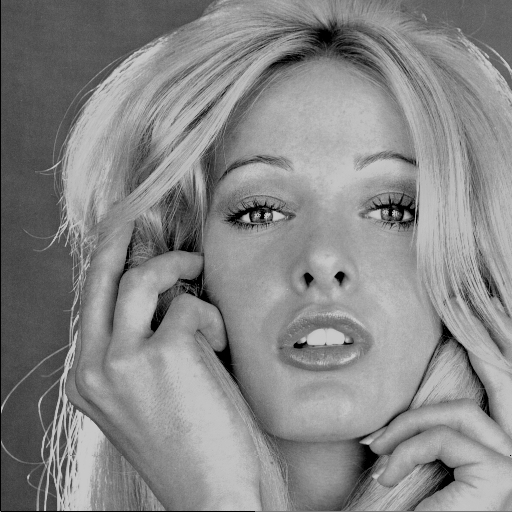
\includegraphics[width=0.2\linewidth]{Graphics/Examples/woman_blonde.png}&
		\includegraphics[width=0.2\linewidth]{Graphics/Examples/mask.tif}\\
		\tiny\texttt{woman\_blonde.tif}&\tiny\texttt{mask.tif}\\
	\end{tabular}
	
	\caption{La imagen y su m\'ascara.}
	\label{fig:woman_blonde}
\end{figure}
Para realizar la restauraci\'on de la imagen se procede como el en siguiente ejemplo:
\begin{lstlisting}
from ImageInpainting import CorruptedImage, read_image_as_mask

# Leyendo la m'ascara y la imagen, luego guardando la imagen corrupta
mask = read_image_as_mask('mask.tif')
im = CorruptedImage('woman_blonde.tif', mask)
im.save('woman_blonde_c.tif')

# Primera restauraci'on con K=10, sqrt_n=5, B=6, epsilon=10000 
im.inpainting(sqrt_n=5, B=6, epsilon=10**4)
im.save('woman_blonde_r1.tif')

# Secunda restauraci'on con K=10, sqrt_n=4, B=7, epsilon=1000000
im.inpainting(sqrt_n=4, B=7, epsilon=10**6)
im.save('woman_blonde_r2.tif')

# Tercera restauraci'on con K=10, sqrt_n=4, B=8, epsilon=100000000 
im.inpainting(sqrt_n=4, B=8, epsilon=10**8)
im.save('woman_blonde_r3.tif')
\end{lstlisting}
La ejecuci\'on de lo anterior genera la versi\'on de la imagen original corrupta seg\'un la m\'ascara, y 3 im\'agenes restauradas usando los par\'ametros que se indican.
\begin{figure}[H]
	\centering
	\begin{tabular}{cccc}
		\includegraphics[width=0.2\linewidth]{Graphics/Examples/woman_blonde_corrupted.tif}&
		\includegraphics[width=0.2\linewidth]{Graphics/Examples/woman_blonde_iteration_1.tif}&
		\includegraphics[width=0.2\linewidth]{Graphics/Examples/woman_blonde_iteration_2.tif}&
		\includegraphics[width=0.2\linewidth]{Graphics/Examples/woman_blonde_iteration_3.tif}\\
		\tiny\texttt{woman\_blonde\_c.tif}&\tiny\texttt{woman\_blonde\_r1.tif}&
		\tiny\texttt{woman\_blonde\_r2.tif}&\tiny\texttt{woman\_blonde\_r3.tif}\\
	\end{tabular}
	\caption{En ese orden: imagen corrupta y las im\'agenes restauradas.}
	\label{fig:inpainting_woman_blonde}
\end{figure}
Finalmente, se ha de destacar que el diseño de la clase \texttt{CorruptedImage} favorece el poder realizar restauraciones consecutivas, cada una usando los resultados de la anterior. Recordemos que cada vez que se llama al m\'etodo de instancia \texttt{inpainting}, el mismo actualiza cada canal de la imagen con los nuevos p\'ixeles restaurados. Esto tiene como consecuencia que en la mayor\'ia de los casos una segunda restauraci\'on tiene mejor calidad que una primera con los mismos par\'ametros. N\'otese que en el ejemplo anterior se realizan 3 restauraciones consecutivas, m\'as adelante se demuestra la efectividad de esta estrategia.

\section{Paralelizaci\'on y herramientas para la experimentaci\'on}

Como se muestra en la figura \ref{fig:final_scheme} del esquema final, se deben realizar $K$ restauraciones del tipo esquema con subim\'agenes, y promediar los resultados en una restauraci\'on final. La forma natural es llevar a cabo las restauraciones iterativamente una despu\'es de la otra. Teniendo en cuenta que los resultados de estas $K$ restauraciones no de penden entre si, surge la idea de poder ejecutarlas de forma concurrente. Por lo tanto se decide aplicar la paralelizaci\'on en ese nivel del esquema. Se utiliz\'o el tipo \texttt{multiprocessing.Pool} el cual modela un contenedor de procesos que se ejecutan en paralelo, el mismo permite agregar procesos nuevos u obtener el resultado de uno que culmina. Se comienza agregando los procesos de las 3 primeras restauraciones de esquema con subim\'agenes. Luego en todo momento se estar\'an ejecutando un m\'aximo de 3 procesos en paralelo, y en la medida que alguno culmine, se almacena su resultado y se agrega el siguiente proceso. As\'i sucesivamente hasta realizar las $K$ restauraciones. Esta estrategia optimiza el tiempo en al rededor de 3 veces m\'as r\'apido que la versi\'on sin concurrencia.

Por otro lado, para facilitar la tarea de experimentaci\'on y comprobaci\'on de la restauraci\'on con determinado volumen de im\'agenes se implement\'o \texttt{experiment.py}, claramente haciendo uso de el m\'odulo \texttt{ImageInpainting}. Dicho programa automatiza el proceso cargar un conjunto im\'agenes, aplicarles la restauraci\'on y almacenar los resultados. El mismo debe proveerse de una descripci\'on simple del experimento a realizar, tal como, la lista de im\'agenes y sus m\'ascaras, cantidad de restauraci\'ones a realizar y qu\'e valores asignar a los par\'ametros en cada caso. Para realizar una evaluaci\'on de los resultados de la experimentaci\'on, se hace uso de otras herramientas que ofrece \texttt{OpenCV}. Tiene una implemenatci\'on para la medida \textbf{PSNR} \cite{enwiki:psnr} en \texttt{cv2.PSNR} que se usar\'a en el Cap\'itulo \ref{chapter:results}. Tambi\'en contiene la funci\'on \texttt{cv2.inpainting} que realiza dos tipos diferentes de restauraci\'on de im\'agenes, los cuales se podr\'an usar para comparar la efectividad de las mismas con la empleada en este trabajo.